\graphicspath{{./tddImages/}}

\section{Game implementation}

\subsection{System overview}
The game can be logically divided into a number of components. These are illustrated in Figure~\ref{overview}. A Model-View-Controller design pattern is used for the game implementation~\citep{Savi07}. The model  consists of a three-dimensional array which is used to store block information, while the view elements are handled by the \emph{OpenGL} \emph{Renderer} class that translates this block information into a visual representation. Finally, the \emph{Game controller} coordinates interaction between these and all other game components. These other components include input handling, which interfaces with the \emph{Feature extraction} and \emph{Gesture recognition} units, as well as a \emph{Game mechanics} module. The \emph{Game mechanics} unit is responsible for manipulating block data in order to implement movement controls. Finally, the \emph{Game version controller} determines which game version should be played and enables and disables the requisite components for each. This unit also handles the tutorial screens and logging of information necessary for later experimental analysis. The visual elements of the game are created using \emph{OpenGL ES}. The menu system and touch events are handled using standard iOS SDK components. The rest of this chapter will discuss these components in more detail. It should be noted, however, that a full discussion of how the gesture engine and in particular, the feature extraction works, has been included in Chapter 4 and as such will not be expanded on here.
\begin{figure}
  \begin{center}
    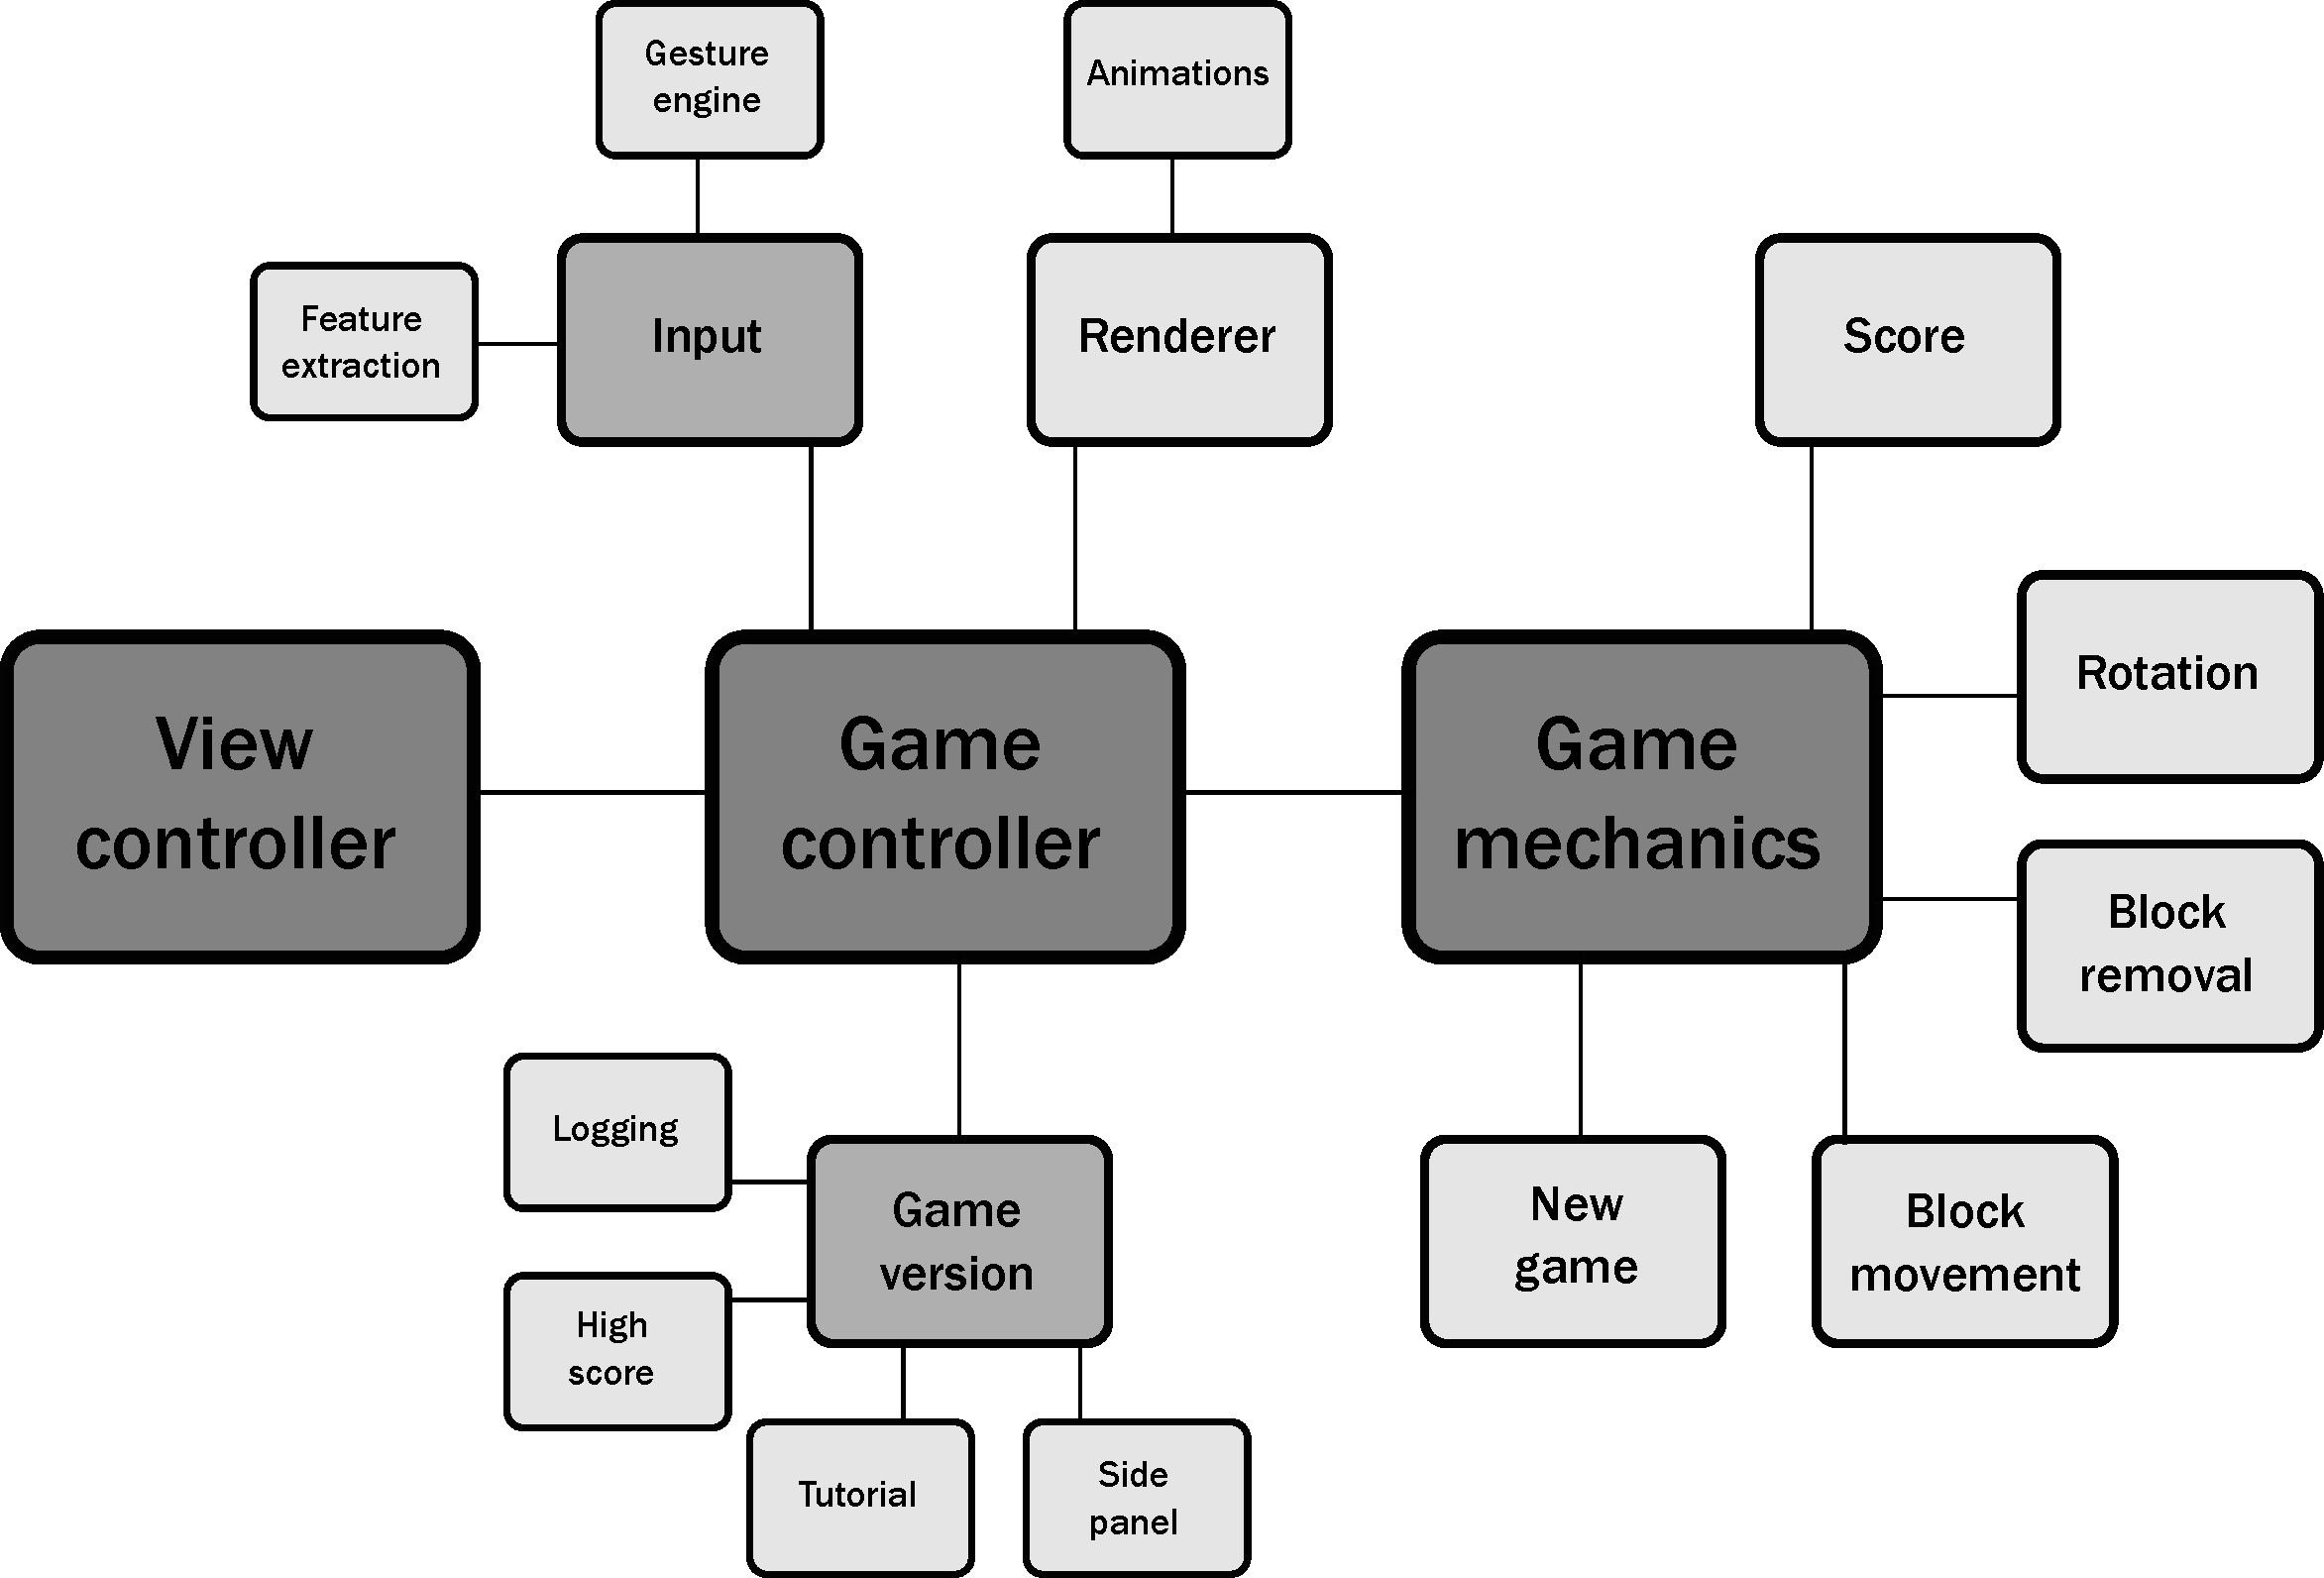
\includegraphics [scale=0.3]{tddOverview.pdf}

  \end{center}
  \caption{Overview of game components and their relation to each other. The use of colour indicates the importance and scope of each component. Dark gray elements are responsible for coordinating a number of other components. Lighter gray items are responsible for the integration of a number of elements within a specific area, while the components in the lightest gray perform a single function and are not responsible for coordinating any of the other named items.}
  \label{overview}
\end{figure}




\subsection{Input events}
Input is received via touch events using the standard touch event handling provided by the iOS SDK. The event handling is broken up into \texttt{touchesBegan}, \texttt{touchesMoved} and \texttt{touchesEnded}. Touch events are handled differently depending on the game version that is being played. The following section provides a brief overview of the input handling and how it is used by each game version.

\subsubsection{Single finger}
\paragraph{touchesBegan}
When a single touch is initiated, the (\emph{x}, \emph{y}) position of the touch is sent to the Game Mechanics module. At this point it is mapped from screen coordinates into the coordinate system used by \emph{OpenGL} drawing (and the block placement array). If the gestural or mixed version is active, this point is also sent to the feature extraction class.

\paragraph{touchesMoved}
In the gestural and mixed version, these points are sent to the feature extraction class. The direct manipulation version ignores these points (as there is no gestural component associated with the game in this case).

\paragraph{touchesEnded}
In all versions a check is done to determine whether the distance between the start and end point is less than 10 pixels. If it is, the movement is considered to be a tap and handled accordingly. The direct manipulation game considers all touch interactions to be taps and thus ignores all points except the start position.

In the gestural and mixed versions, the point is sent to the feature extraction endpoint method. The gesture engine is then passed this data and either returns which gesture is recognised or \texttt{null} if no gesture is found.

\subsubsection{Two fingers}
Multi-touch is disabled in the direct manipulation version as all controls are handled via buttons, therefore this section refers to the gestural and mixed versions only.

The start and end point of the touch interaction are recorded and sent to Game Mechanics where the angle of rotation is determined. This angle is returned and set as the angle of rotation for the renderer class (in order to visually rotate the shape).

\subsubsection{Three fingers}
As mentioned above, multi-touch is disabled in the direct manipulation version. In the other two game versions, the touches are ignored unless they fall within the 100 leftmost pixels of the screen. In this case, the direction of the touch interaction is determined and passed to the method that handles the hiding and redisplay of the gesture hint panel (See Section 3.3.7).  

\subsection{Data organisation}
The primary data handled within the game is the information associated with each block. While touch information is also stored, the description of how this is done is included in the Gesture Engine design chapter. The following section describes how block data is stored.

\subsubsection{Block objects}
Each on screen block has an associated block object. This object stores the following information:
\begin{itemize}
\item (\emph{x}, \emph{y}, \emph{z}) position
\item Colour
\item (\emph{x}, \emph{y}, \emph{z}) position and increment for translation
\end{itemize}

\subsubsection{Block placement array}
Pointers to these block objects are stored in a three-dimensional array that mimics their onscreen arrangement. The array is of size $11 \times 11 \times 11$. As the centremost block on screen is located, in visual coordinates, at position (0, 0, 0), this block is positioned at index (5, 5, 5) within the array. Thus, in order to convert array indices to visual coordinates, -5 is added to the array coordinates. When blocks are removed, their position in the array is set to \texttt{null}.

\subsubsection{Drawing array}
Pointers to all visible blocks are also added to a second linear array. A pointer to this array is passed to the renderer class so that each block can be drawn.

\subsection{File formats}
Logging information is recorded during game-play for later analysis. In addition, the top high score is also recorded. The format of these files is described below.

\subsubsection{High score}
The current score is checked against the high score at the end of each game, as well as when a new game is started manually by the player. If the new score is greater than the previous high score, this new score is written out to a file as a string. This overwrites the previous high score.

\subsubsection{Logging information}
Information on the order in which the games are played, as well as which controls were used and how often, is recorded for each gaming session. Each session appends this data to the end of a file in the following format: \\
\indent \indent \texttt{Date and time} \\
\indent \indent \texttt{Game version number 1} \\
\indent \indent \texttt{Control data} \\
\indent \indent \texttt{Game version number 2} \\
\indent \indent \texttt{Control data} \\
\indent \indent \texttt{Game version number 3} \\
\indent \indent \texttt{Control data} \\
Game version number refers to a number between 0 and 2 which specifies which game was played. The numbers represent the following game conditions:
\begin{center}
\begin{tabular}{c c c}
  0 - Direct manipulation interface & 1 - Gestural interface & 2 - Mixed interface \\
\end{tabular} \end{center} 
Control data refers to the information on the number of times each game control was used. This is organised as follows: \\
\indent \indent \texttt{Control number: Number of times used} \\
The control numbers range from 0 to 12 and correspond to the movement techniques as shown in Table~\ref{controlNo}.
\begin{table}
\centering %
\begin{tabular*}{\textwidth}{c | c c c c c c c }

\hline	
  Number & 0 & 1 & 2 & 3 & 4 & 5 & 6 \\
  Control & Row left & Row right & Column up & Column down & Forward & Backward & Swap left  \\
  \hline
  Number & 7 & 8 & 9 & 10 & 11 & 12 \\
  Control & Swap right & Swap up & Swap down & Move together & Rock shape & Rotate \\
\hline  
\end{tabular*}
\caption{Control numbers and their corresponding movement controls}
\label {controlNo}
\end{table}

\subsection{Game mechanics}
This module is responsible for determining block movements and removal. The implementation of these controls is described in more detail below.

\subsubsection{Block identification}
As all block information is stored in a three-dimensional array that mirrors placement on screen, a block's screen position can be used to determine its position within the array. However, as the contents of the array are not rearranged when a rotation of the shape takes place, the currently visible face may not correspond to the frontmost elements in the array. For this reason, the correct coordinates need to be calculated from the screen coordinates. This is done using rotational matrices corresponding to the \emph{x}-, \emph{y}- and \emph{z}-axes. A description of how the coordinates of these axes are calculated is included in a subsection below. 

The mapped input coordinates are first checked to ensure they fall within the onscreen range of the shape. The following matrix multiplication is then applied:
\begin{displaymath}
	\begin{bmatrix}
		X' \\ Y' \\ Z'
	\end{bmatrix} = 
	\begin{bmatrix}
		x_{0} & x_{1} & x_{2} \\
		y_{0} & y_{1} & y_{2} \\
		z_{0} & z_{1} & z_{2} 
	\end{bmatrix}
	\begin{bmatrix}
		X \\ Y \\ Z
	\end{bmatrix}
	+ 5
\end{displaymath}
where $X$, $Y$ and $Z$ are the input \emph{x} and \emph{y} coordinates and $Z$ is set to 5 (as this is the frontmost block at these coordinates). The $3 \times 3$ matrix stores the current orientation of the axes. 5 is added to the result as view coordinates range from -5 to 5, while array indices begin at 0. This entire operation maps the view screen coordinates to array indices.

If the block at that position does not exist because the user has removed it from screen, and is thus attempting to interact with the currently visible block beneath it, the values are recomputed with $Z$ set to 4. The value of $Z$ continues to be decremented until a valid block is found or until the $Z$ value is outside the valid range of block positions. If a block is found, a pointer to it is returned, otherwise \texttt{null} is returned.


\subsubsection{Movement of rows and columns}
For the purpose of this explanation, a row and column are defined as follows:

\begin{itemize}
	\item {\bf Row:} All blocks which share a common \emph{y} value. In addition, they should be equidistant from the \emph{y}-axis. 
	\item {\bf Column:} All blocks which share a common \emph{x} value. In addition, they should be equidistant from the \emph{x}-axis. 
\end {itemize}

The manipulation of columns and rows is fairly similar, except that in the case of rows the \emph{y} coordinate is held constant, while with columns the \emph{x} coordinate remains the same. For this reason, the description below refers to the implementation of \emph{Left}, \emph{Right}, \emph{Up} and \emph{Down} operations. The following equation describes this operation mathematically:\\
\begin{displaymath}V(Rot(P_{x, y, z}))  = V(P_{x, y, z})  \mbox{ where}\end{displaymath}
\footnotesize
\begin{align*}
\begin{array}{ l l l l l l }
		Rot_{Left}(P_{x,y,z}) & = & \left\{ 
			\begin{array}{l l l}
			  P_{x-1,y,z^{\prime}} & \quad \mbox{if } P_x > -z^{\prime} \\ 
			  P_{-z^{\prime},y,z-1} & \quad \mbox{if } P_z > -z^{\prime} \\ 
			  P_{x+1,y,-z^{\prime}} & \quad \mbox{if } P_x < z^{\prime} \\ 
			  P_{z^{\prime},y,z+1} & \quad \mbox{if } P_z < z^{\prime} \\ 
			 \end{array} \right. 
			& Rot_{Right}(P_{x,y,z})& = & \left\{  \begin{array}{l l l}
			  P_{x+1,y,z^{\prime}} & \quad \mbox{if } P_x < z^{\prime} \\ 
			  P_{z^{\prime},y,z-1} & \quad \mbox{if } P_z > -z^{\prime} \\ 
			  P_{x-1,y,-z^{\prime}} & \quad \mbox{if } P_x > -z^{\prime} \\ 
			  P_{-z^{\prime},y,z+1} & \quad \mbox{if } P_z < z^{\prime} \\ 
			 \end{array} \right. \\
			& & & & & \\
		Rot_{Down}(P_{x,y,z}) & = & \left\{ 
			\begin{array}{l l l}
			  P_{x,y-1,z^{\prime}} & \quad \mbox{if } P_y > -z^{\prime} \\ 
			  P_{x,-z^{\prime},z-1} & \quad \mbox{if } P_z > -z^{\prime} \\ 
			  P_{x,y+1,-z^{\prime}} & \quad \mbox{if } P_y < z^{\prime} \\ 
			  P_{x,z^{\prime},z+1} & \quad \mbox{if } P_z < z^{\prime} \\ 
			\end{array} \right. 
			& Rot_{Up}(P_{x,y,z})& = & \left\{  \begin{array}{l l l}
			  P_{x,y+1,z^{\prime}} & \quad \mbox{if } P_y < z^{\prime} \\ 
			  P_{x,z^{\prime},z-1} & \quad \mbox{if } P_z > -z^{\prime} \\ 
			  P_{x,y-1,-z^{\prime}} & \quad \mbox{if } P_y > -z^{\prime} \\ 
			  P_{x,-z^{\prime},z+1} & \quad \mbox{if } P_z < z^{\prime} \\ 
			 \end{array} \right. \\
	\end{array} \\
\end{align*}
\normalsize
where $V$ is the view screen to array coordinates transform described above, $P$ is the three-dimensional position of a cube in view screen coordinates, $Rot$ describes the operations used to rotate around the specific layer in the required direction and $z^{\prime}$ is the maximum extent in the \emph{z} direction.

Thus, the coordinates of the block touched by the user are passed to the block identification method described above. This checks whether this is a valid block and returns a pointer to this block in the array. It also sets the current \emph{z} value for use with the later manipulations as this defines which layer within the shape the movement is being applied to. As the application of one of these commands may actually require rotation around some other axis than the one provided by view screen coordinates (due to rotation of the shape), visual coordinates, rather than array coordinates, are used to iterate through the row. That is, the visual coordinates are manipulated and then mapped back to array coordinates (using the block identification method) in order to adjust the position of block objects. 

The coordinates stored within each block object as well as their position in the array are updated using this method. Positions with a \texttt{null} value are also translated in this manner.

\subsubsection{Movement along the \emph{z}-axis}
The implementation of the \emph{Forward} and \emph{Backward} commands is similar to that for rows and columns. In this case, the visual \emph{x} and \emph{y} coordinates are held constant, while the \emph{z} coordinate is changed. These visual coordinates are mapped to array coordinates and the block objects moved accordingly. This is illustrated mathematically below:
\begin{displaymath}
	\begin{array}{l l l}
		\mbox{Forward:} & V(P_{x, y, (z+1) \% z^{\prime}})  = V(P_{x, y, z}) & x = x_c, y = y_c \\
		& & \\
		\mbox{Backward:} & V(P_{x, y, (z-1) \% z^{\prime}})  = V(P_{x, y, z}) & x = x_c, y = y_c \\
	\end{array}
\end{displaymath}
where $V$ is the view screen to array coordinates transform described above, $P$ is the three-dimensional position of a cube in view screen coordinates, $x_c$ and $y_c$ are constants and $z^{\prime}$ is the maximum extent in the \emph{z} direction.

\subsubsection{Swapping of blocks}
In order to determine which blocks are to be swapped, the array coordinates for the selected block are calculated. Visual coordinates of this block are then manipulated in order to determine the neighbour with which the block should be swapped. These are then mapped to array coordinates and the position of the two blocks is updated.

\subsubsection{Moving blocks together}
When a \emph{Move together} command is executed the following three steps are completed in order to move all blocks in towards the view screen origin, thus removing any gaps between them caused by the removal of blocks. The first step involves checking the \emph{z} array coordinate of a block and the block behind it. The \emph{z} coordinate of the previous block is determined as follows:
\[z_{prev} = \left\{ 
\begin{array}{l l}
  z - 1 & \quad \mbox{if }z > 0 \\
  z + 1 & \quad \mbox{if }z < 0 \\ 
\end{array} \right. \]
If the current block has a \emph{z} coordinate of 0, it is ignored. The same procedure is then followed for the \emph{x}- and \emph{y}-axes. This process is applied from the origin outward to ensure that all blocks are moved as far in as possible. This serves to move all blocks in towards the origin, compacting them in the process. Figure~\ref{ss:moveIn} illustrates the effects of this command.

\begin{figure}
  \centering
  \subfloat[Initial shape with blocks removed]{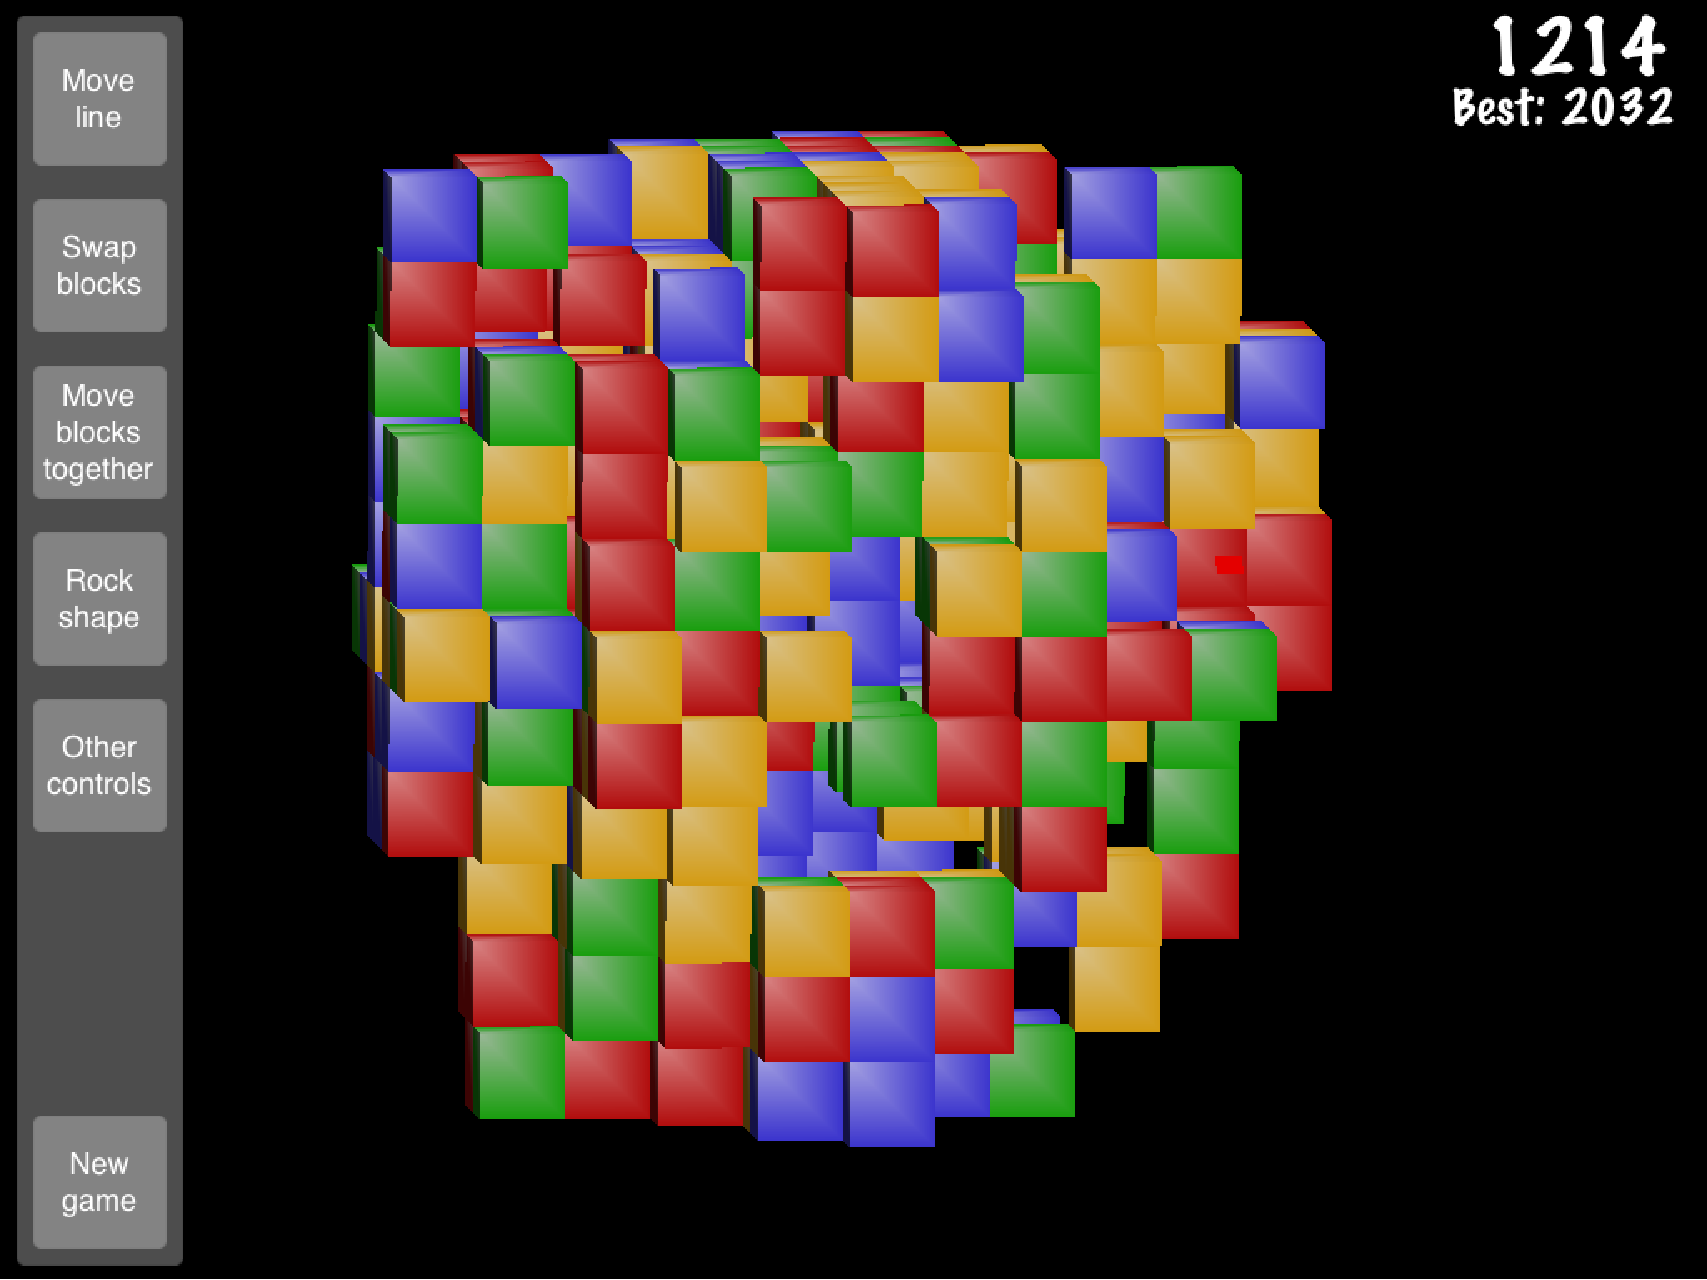
\includegraphics[scale=0.2]{moveB.pdf}}       \hspace{20pt}   \vspace{10pt}       
  \subfloat[Shape after \emph{Move together} command]{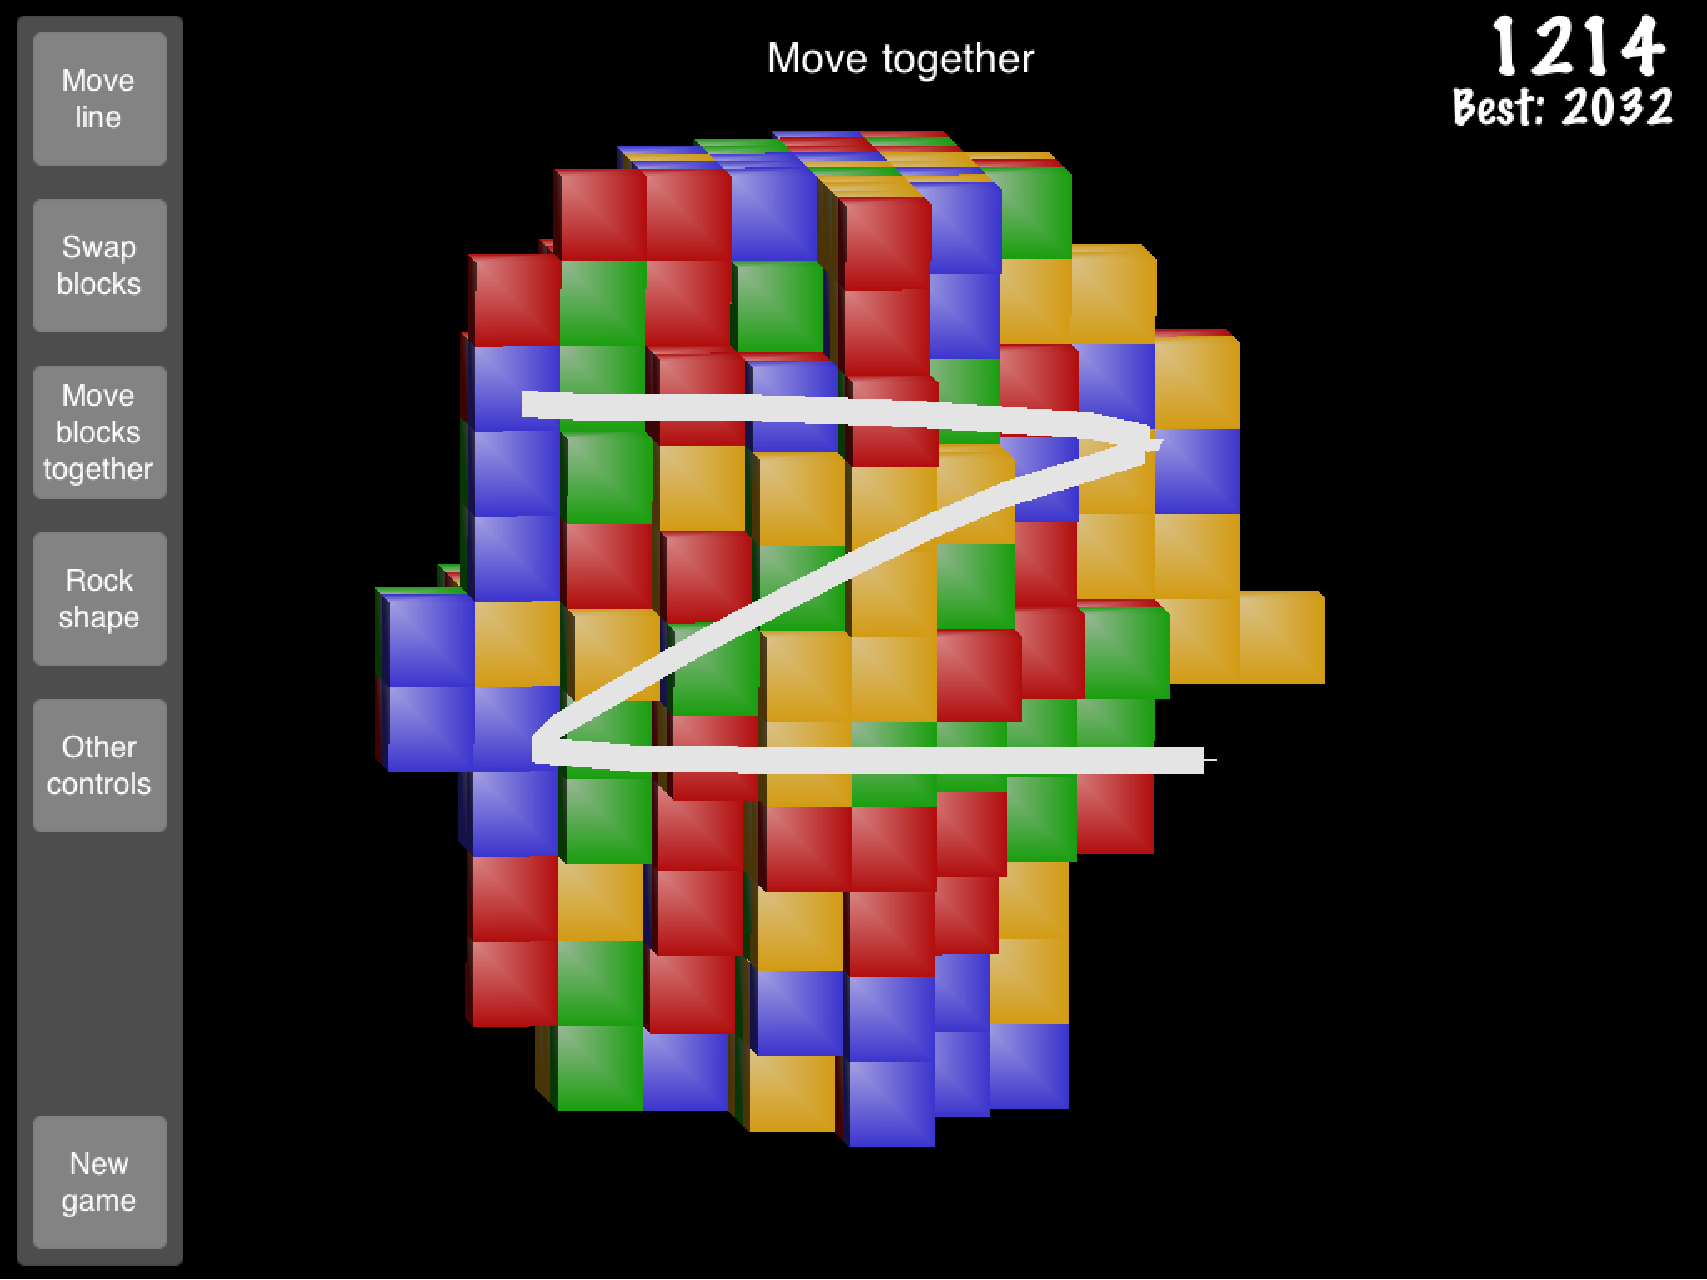
\includegraphics[scale=0.2]{moveA.pdf}} \hspace{20pt}
  
   \caption{Screenshots of the game illustrating the \emph{Move together} command.}
  \label{ss:moveIn}
\end{figure}


\subsubsection{Block removal}
When a block is set to be removed, it recursively calls a method on its neighbours in order to determine whether they are of the same colour. Blocks are considered to be neighbours if they have at least one face touching. If a block is the same colour, it sets a check variable (so that it is not removed more then once), adds itself to a list of blocks to be removed and calls the removal method on its neighbours. This continues until no more blocks of the same colour can be found. If the removal list has a length of 3 or more, the blocks in this list are removed from both the block position array and the drawing array.

\subsubsection{Shape rotation}
Rotations are primarily implemented in the \emph{OpenGL} renderer, however, the game mechanics module is also required to keep track of rotations in order to correctly identify blocks within the placement array. 

In order to correctly map visual coordinates to array coordinates, it is necessary to keep track of the orientation of each axis. This is done by recording the orientation of each axis as a column vector and then multiplying them with the appropriate rotational matrix every time a rotation is needed. As rotation is only possible in one direction at a time, this is a fairly simple procedure. The rotational matrices for rotation around the \emph{x}- and \emph{y}-axes are shown below:

\begin{eqnarray*}
R_x(\theta) & = & \begin{bmatrix} 1 & 0 & 0 \\
0 & \cos \theta & -\sin \theta \\
0 & \sin \theta & \cos \theta \end{bmatrix} \\
R_y(\theta) & = & \begin{bmatrix} \cos \theta & 0 & \sin \theta \\
0 & 1 & 0 \\
-\sin \theta & 0 & \cos \theta \end{bmatrix}
\end{eqnarray*}


\subsubsection{New game}
When the \emph{New game} button is selected a number of steps are taken to return the game to its original state. This requires reseting the block array as well as the rotational coordinates of the axes in both the renderer and the game mechanics module.

The block placement array is iterated through. In order to prevent unnecessary reallocation of memory, any positions which already hold block objects simply have the block object passed a new randomly generated colour. Indexes with a \texttt{null} value are assigned a new block object. The drawing array is cleared and these new objects added. Finally, the rotational matrix in the renderer and the axes in game mechanics are reset. The score is also checked to determine whether it is better than the previous highest score. If it is, the high score value is changed. The score is then reset to 0. 


\subsection{Game rendering}
Rendering of the blocks that compose the overall shape as well as touch events created by the user is done using \emph{OpenGL ES}. An orthographic projection was used to display the blocks. Simple lighting was also implemented in order to aid the illusion of three-dimensionality. In order for the lighting to best illustrate the three-dimensional nature of each cube, surface, rather than vertex normals are required. For this reason, cubes are drawn using \texttt{GL\_TRIANGLES} rather than \texttt{GL\_TRIANGLE\_STRIP}. The shape is also rotated by 5 degrees in the \emph{x} and \emph{y} directions so that additional shape faces are visible to provide depth cues. The matrix used to represent the orientation of a block is translated to the position of each block (specified in the array containing block objects). This is then drawn with the colour listed in each block object. 

A pointer to an array of all the current touch points is also passed to the renderer. These are then linked and drawn in white. When the touch ends, this array is cleared. When a gesture is not recognised, a flag is set, and the renderer draws this line in red.

\subsubsection{Animations}

\paragraph{Rotation}
Since applying an \emph{OpenGL} rotation also rotates the coordinate system in use, a separate transform matrix is kept. Rotations are then applied to this matrix which is then loaded as the current matrix. In order to do this, an instance of the built-in type, \texttt{CATransform3D}, is used to record the current orientation of a cube. The required rotation is then incrementally applied to this matrix. This is done separately along the \emph{x}- and \emph{y}-axes. The incremental nature of the rotation is used in order to produce a rotational animation effect.

\paragraph{Translation}
Most block movement operations require some form of animation. A simple translation is used to achieve this effect. Blocks are incrementally moved from their original position to their new position. Each block object contains additional variables used to determine their position during this gradual translation. When a block is marked for translation, the new position is passed in and the increment determined. These blocks are then removed from the main drawing array and placed in a separate translation array. The renderer then calls the translation method within each block until it has reached its new position. At this point, the block is removed from the translation array and re-inserted into to the main drawing array. In this way, it is possible to translate multiple blocks in different directions simultaneously.

\subsection{Interface elements}
Each game version has an associated side panel. The function of this panel, however, depends on the interface in use. The side panel can be hidden by completing a three-finger swipe towards the left edge of the screen. A swipe starting at the left edge and moving inward redisplays this panel. An animation is used when moving the panel in and out. Figure~\ref{interfaces} shows all three interface versions, as well as a sample side panel for each case.
\begin{figure}[h]
  \centering
  \subfloat[Direct manipulation interface]{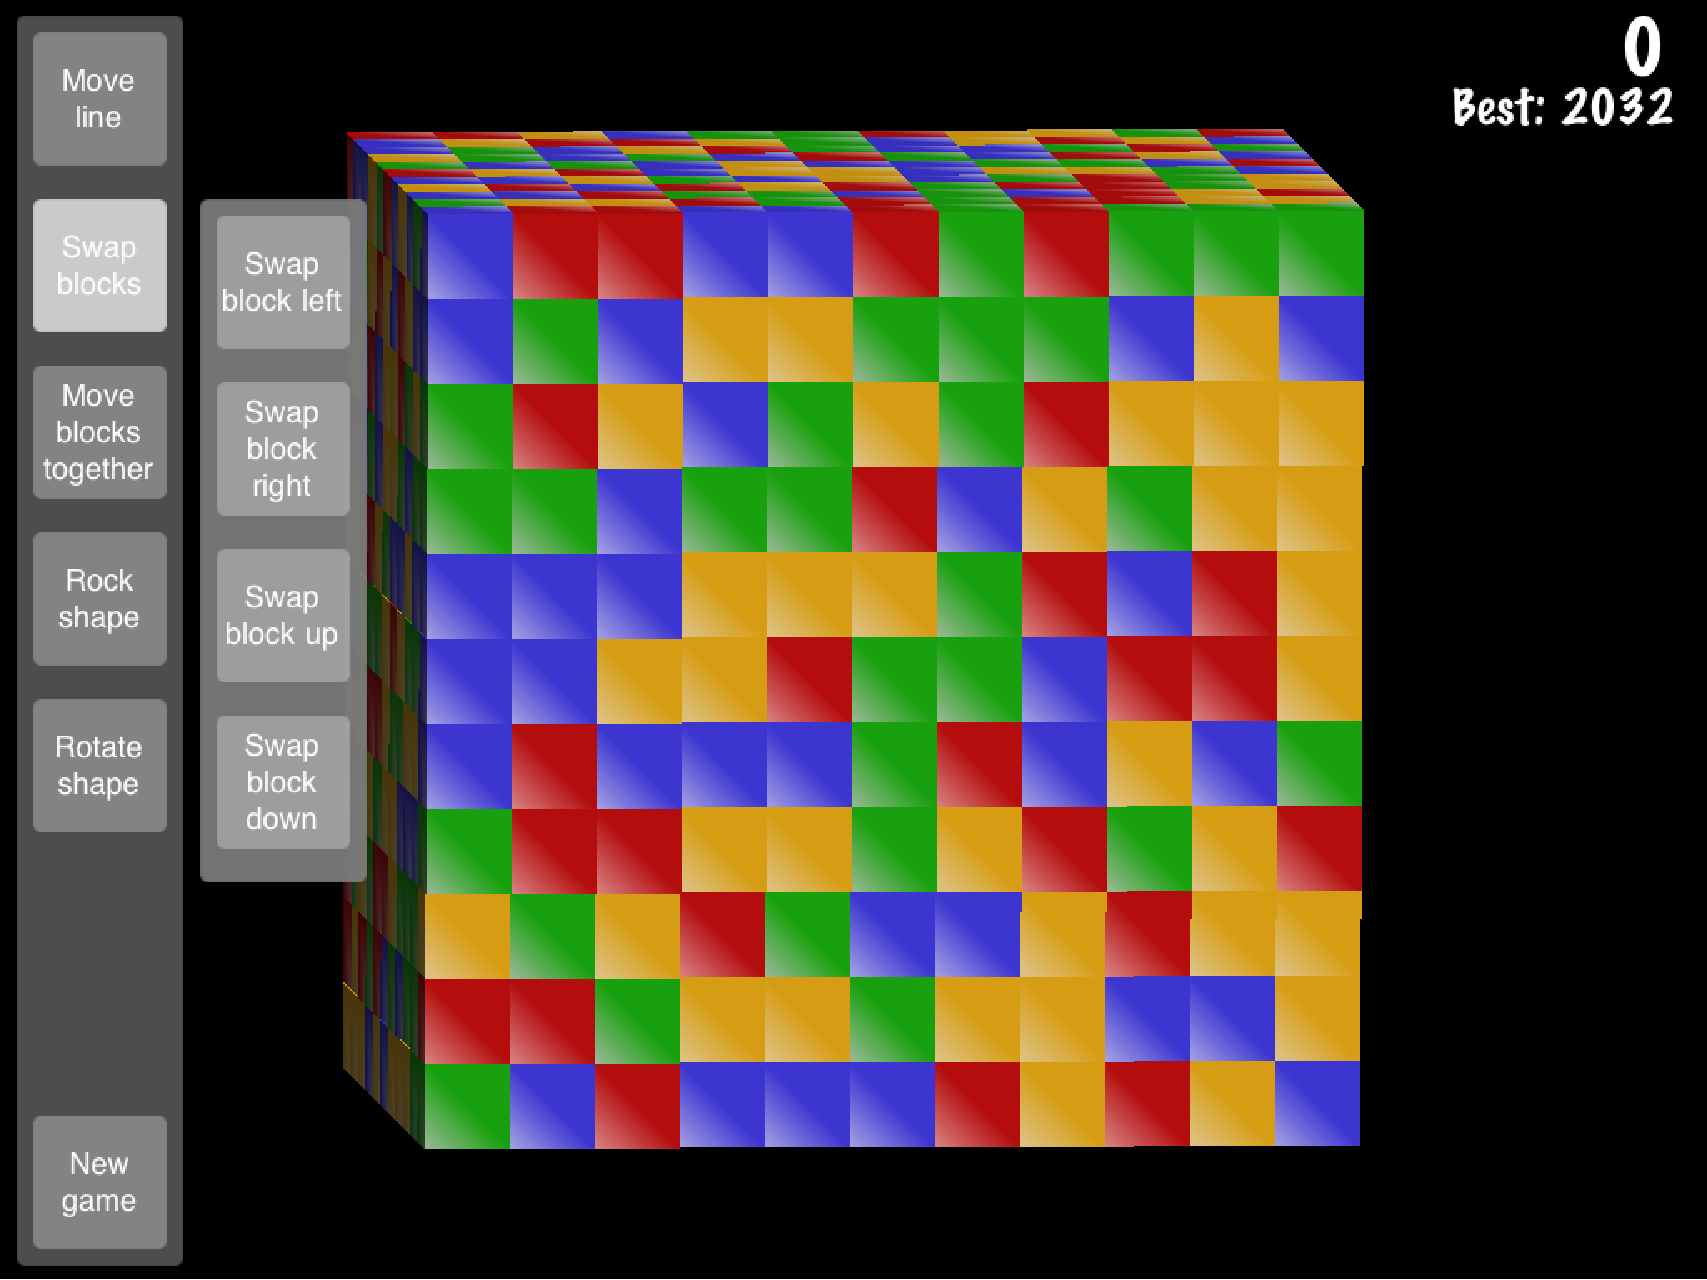
\includegraphics[scale=0.2]{dmSS.pdf}}       \hspace{20pt}   \vspace{10pt}       
  \subfloat[Gestural interface]{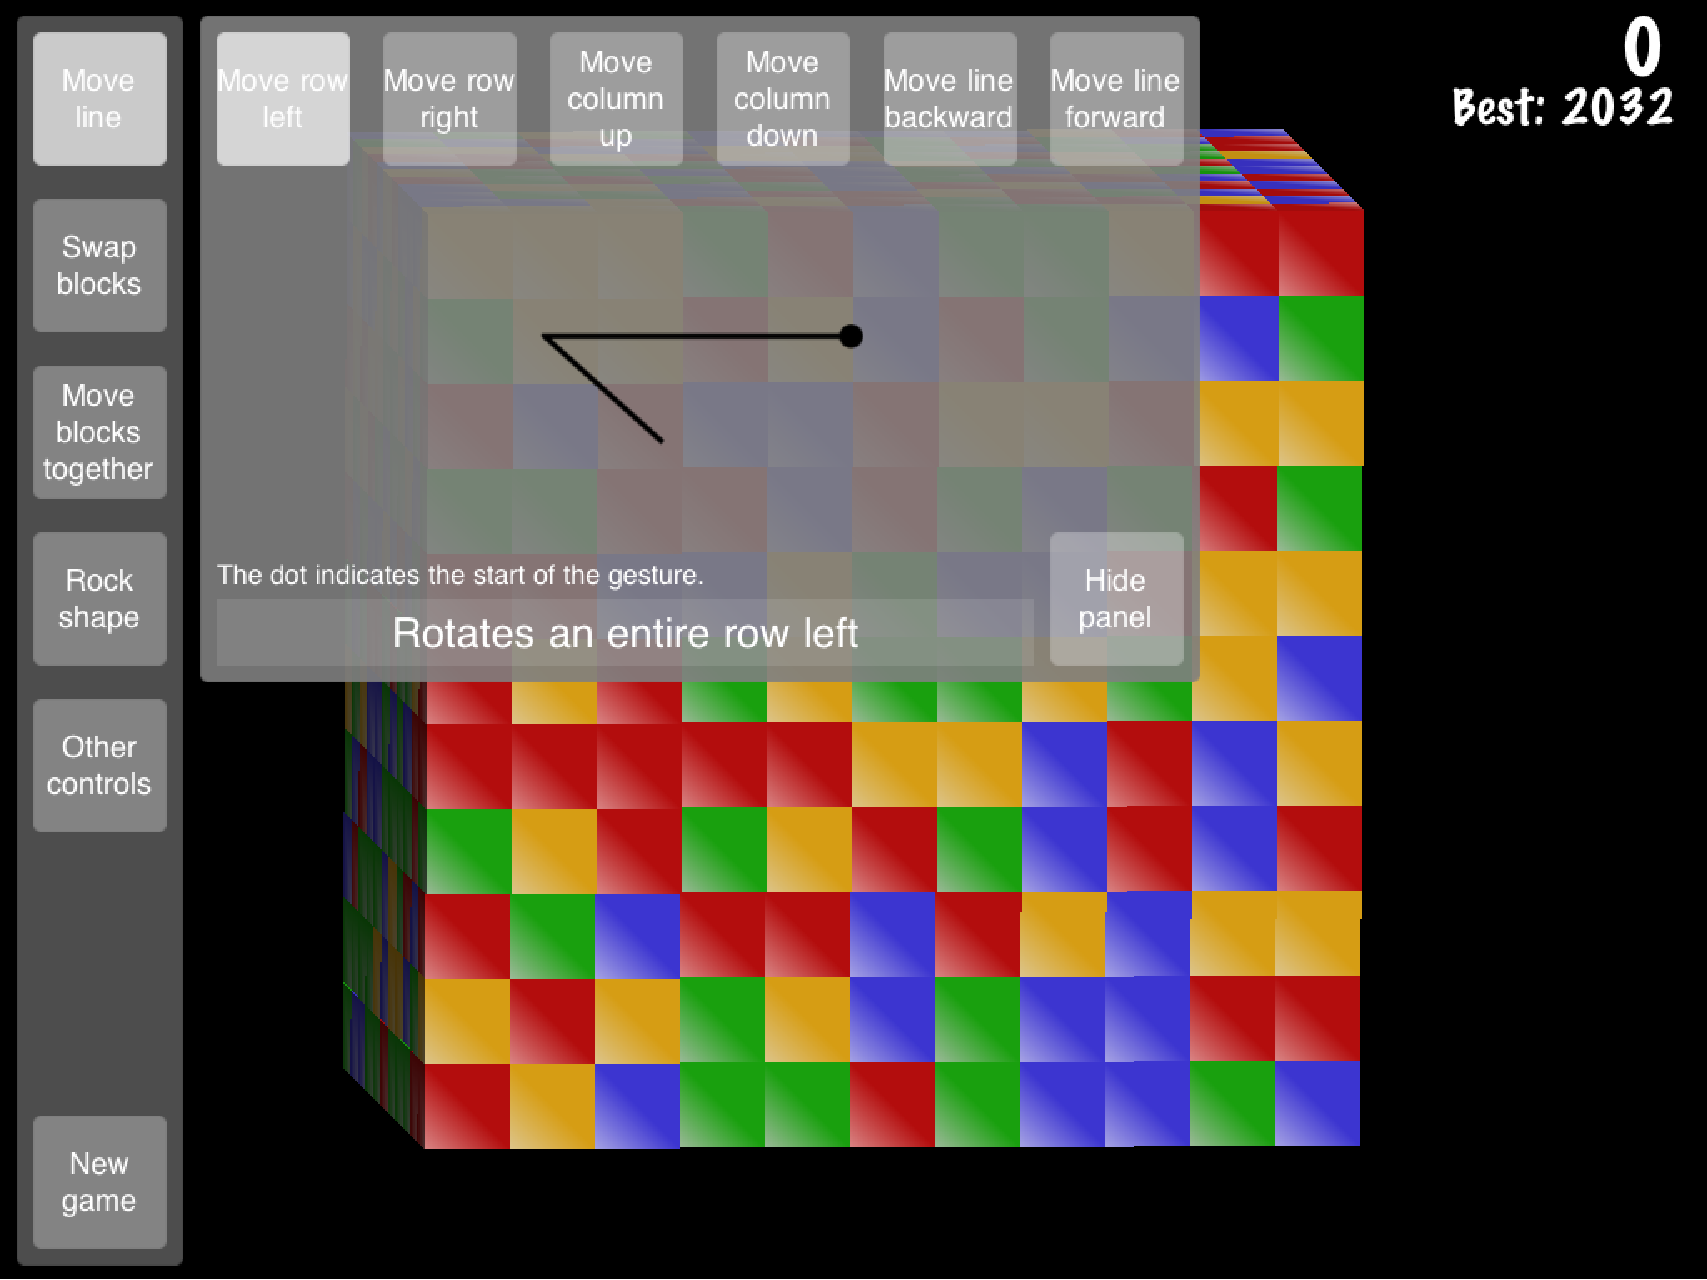
\includegraphics[scale=0.2]{gestureSS.pdf}} \hspace{20pt}
  \subfloat[Mixed interface]{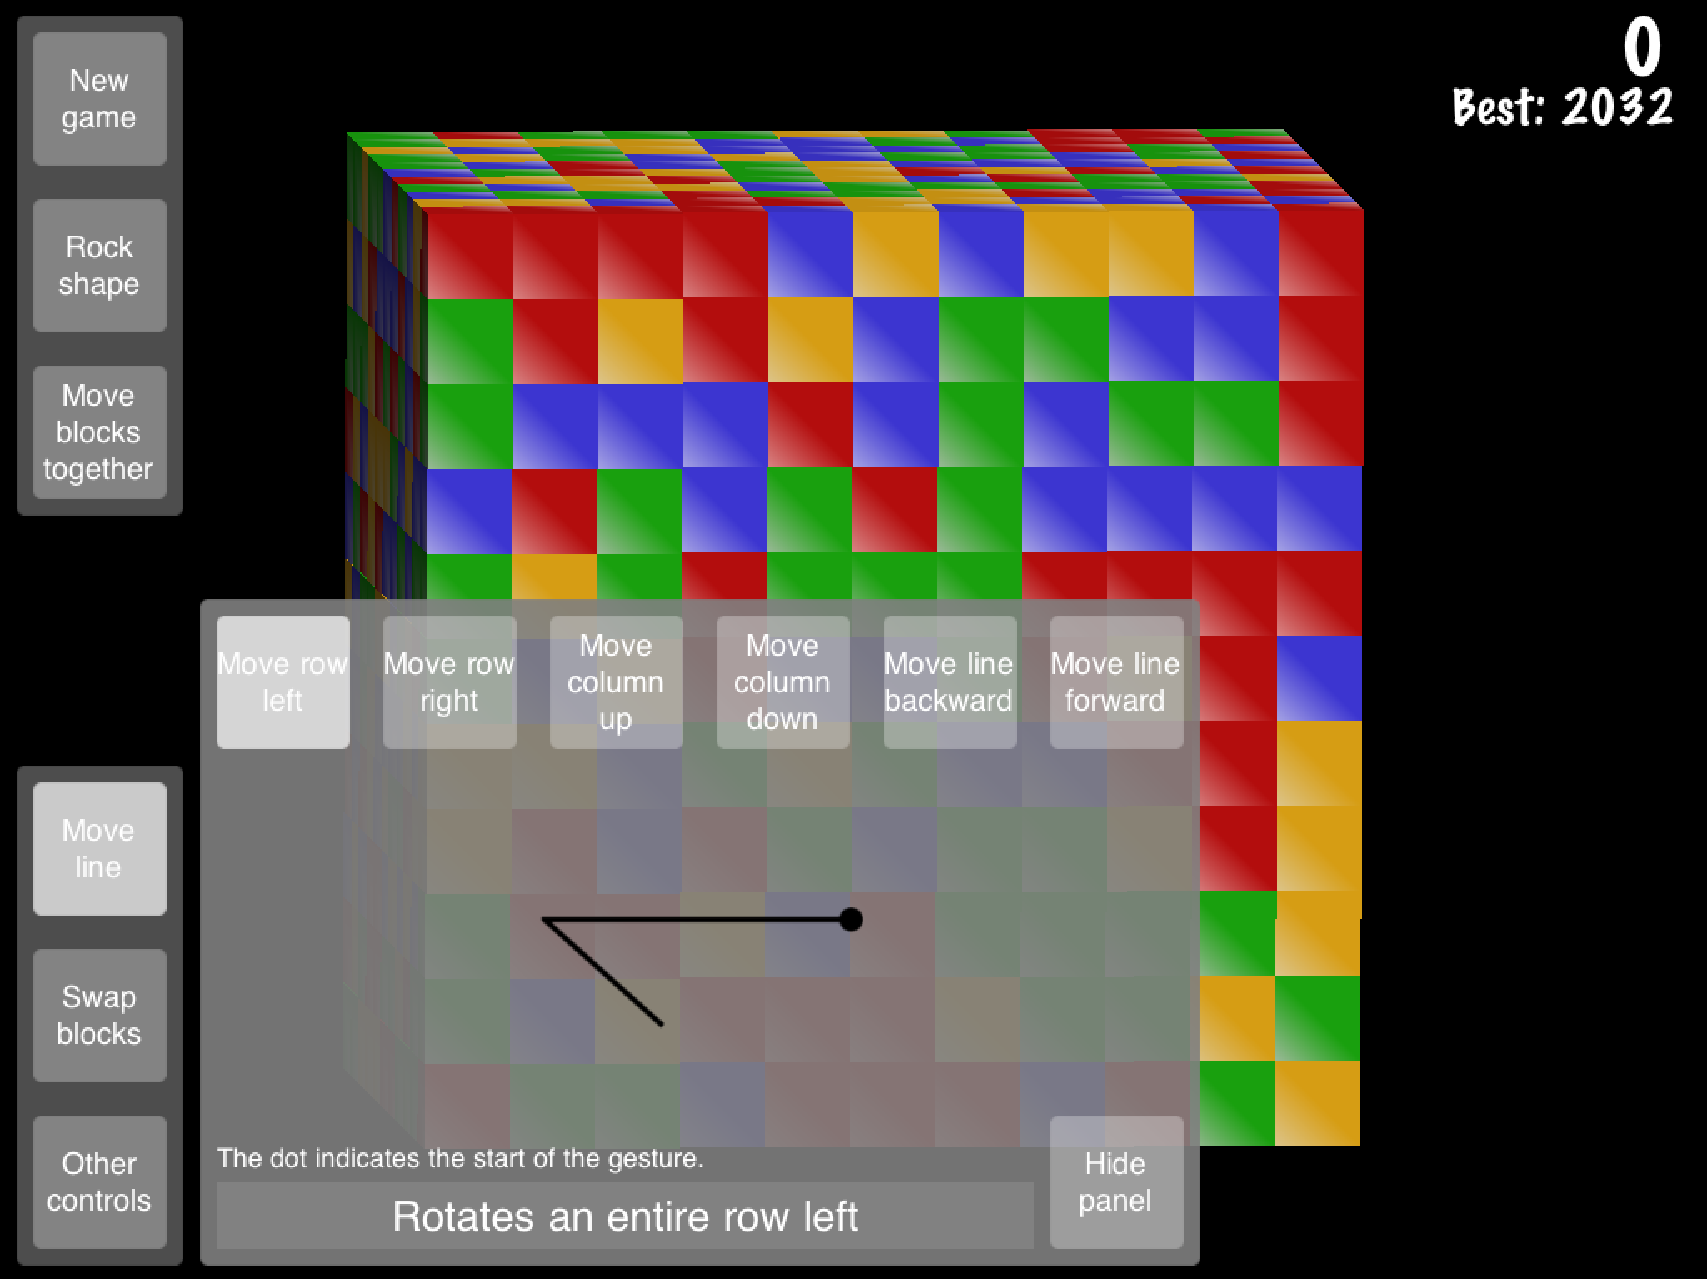
\includegraphics[scale=0.2]{mixedSS.pdf}} \hspace{20pt}   
   \caption{Screenshots of the three interface versions. A side menu has been activated in each case.}
  \label{interfaces}
\end{figure}

\subsubsection{Gesture hint panel}
This panel is used to display information on the possible gestures. Selecting a button displays a second panel which illustrates the gesture as well as its function. This panel is visible in the gestural and mixed game versions.

\subsubsection{Control button panel}
This panel is used in the direct manipulation and mixed game versions. It contains buttons that can be used to control block manipulation. Once a button has been selected it remains selected until either a new button is chosen or it is unselected by the user. If a button is selected, all interaction with the shape is interpreted as applications of the selected control.

\subsection{Game version controller and sequence}
As there are multiple game versions, a mechanism is needed to transition between the interfaces of each. In addition, various components need to be enabled or disabled depending on the active game version. Game-play consists of a tutorial session followed by the three game versions. This is handled as described below.

\subsubsection{Tutorial}
During the tutorial the player is shown an image of the gesture they are to practice. They are then asked to draw this gesture ten times. Once they have successfully completed ten gestures (that is, the gesture they have drawn has been recognised correctly ten times), the next gesture is displayed and the process repeated. This is done for all gestures used in the gestural and mixed interface versions of the game.

The tutorial screen drawing is handled by the renderer. During this stage the block drawing array is empty so only the user's touches are drawn. These touches are passed to the gesture recognition engine and handled accordingly. Once all gestures have been tested in this manner, control is passed to the game version controller.

\subsubsection{Game choice}
Once the tutorial section is complete, a game description screen is displayed. This contains information on what the game entails. Control is then passed to a method which determines which game version should be played. This is done by selecting a random number between 0 and 2. The numbers represent the following game conditions:
\begin{center}
\begin{tabular}{c c c}
  0 - Direct manipulation interface & 1 - Gestural interface & 2 - Mixed interface \\
\end{tabular} \end{center} 
This number is checked against a \texttt{BOOL} array of size 3. If the element at this index is set to \texttt{True}, the process is repeated until a number is chosen that corresponds to a game version that has not yet been played. The array is then updated and the setup for that game version is completed. This entails enabling and disabling menu or hint panels and the accepted gestures for that game version. Table~\ref{diffVer} illustrates the components used for each game version. 

\begin{table}

\centering
\begin{tabular}{l | p{3cm} | p{3cm} | p{3cm}}
\hline
 Interface version &  Gestures enabled &  Hint panel &  Button panel \\
\hline
\textit{Direct manipulation} & None & Hidden & Visible \\[2pt]
\hline
\textit{Gestural} & All enabled & Visible & Hidden \\[2pt]
\hline
\textit{Mixed} & All enabled apart from \emph{Rock shape} and \emph{Move together} & Visible but without buttons for \emph{Rock shape} and \emph{Move together} & Visible but only contains the \emph{Rock shape} and \emph{Move together} buttons along with the \emph{New game} button \\[2pt]
\hline
\end{tabular}
\caption{Overview of the interface and interaction elements available in each game version}
\label {diffVer}
\end{table}

Once the game has been setup, the user plays it for 7 minutes. At this point a timer interrupts game-play and the user is presented with the instructions for the next game version. Logging information is also written to file and the timer is reset. The logging information is described in more detail above. Once all three games have been played, a game end screen is displayed.



